\documentclass[a4paper]{article}
\usepackage{geometry}
\geometry{left=2.54cm,right=2.54cm,top=2.54cm,bottom=2.54cm}
\usepackage{amsmath}
\usepackage{amsfonts}
\usepackage{graphicx}
\usepackage{booktabs}
\usepackage{indentfirst}
\setlength{\parindent}{2em}
\usepackage{url}
\usepackage{fancyhdr}
\usepackage{lastpage}
\usepackage{float}
\pagestyle{fancy}
\lhead{Team \#58893}
\rhead{Page \thepage\ of \pageref{LastPage}}
\cfoot{}
\usepackage{hyperref}
\usepackage{setspace}
\usepackage{pdfpages}
\usepackage{listings}
	\lstset{
		basicstyle=\tt,
		%行号
		numbers=left,
		rulesepcolor=\color{red!20!green!20!blue!20},
		escapeinside=``,
		xleftmargin=2em,xrightmargin=2em, aboveskip=1em,
		%背景框
		framexleftmargin=1.5mm,
		frame=shadowbox,
		%背景色
		backgroundcolor=\color[RGB]{245,245,244},
		%样式
		keywordstyle=\color{blue}\bfseries,
		identifierstyle=\bf,
		numberstyle=\color[RGB]{20,20,20},
		commentstyle=\it\color[RGB]{96,96,96},
		stringstyle=\rmfamily\slshape\color[RGB]{128,0,0},
		%显示空格
		showstringspaces=false,
		breaklines=true
	}

\usepackage{xcolor}

\begin{document}
	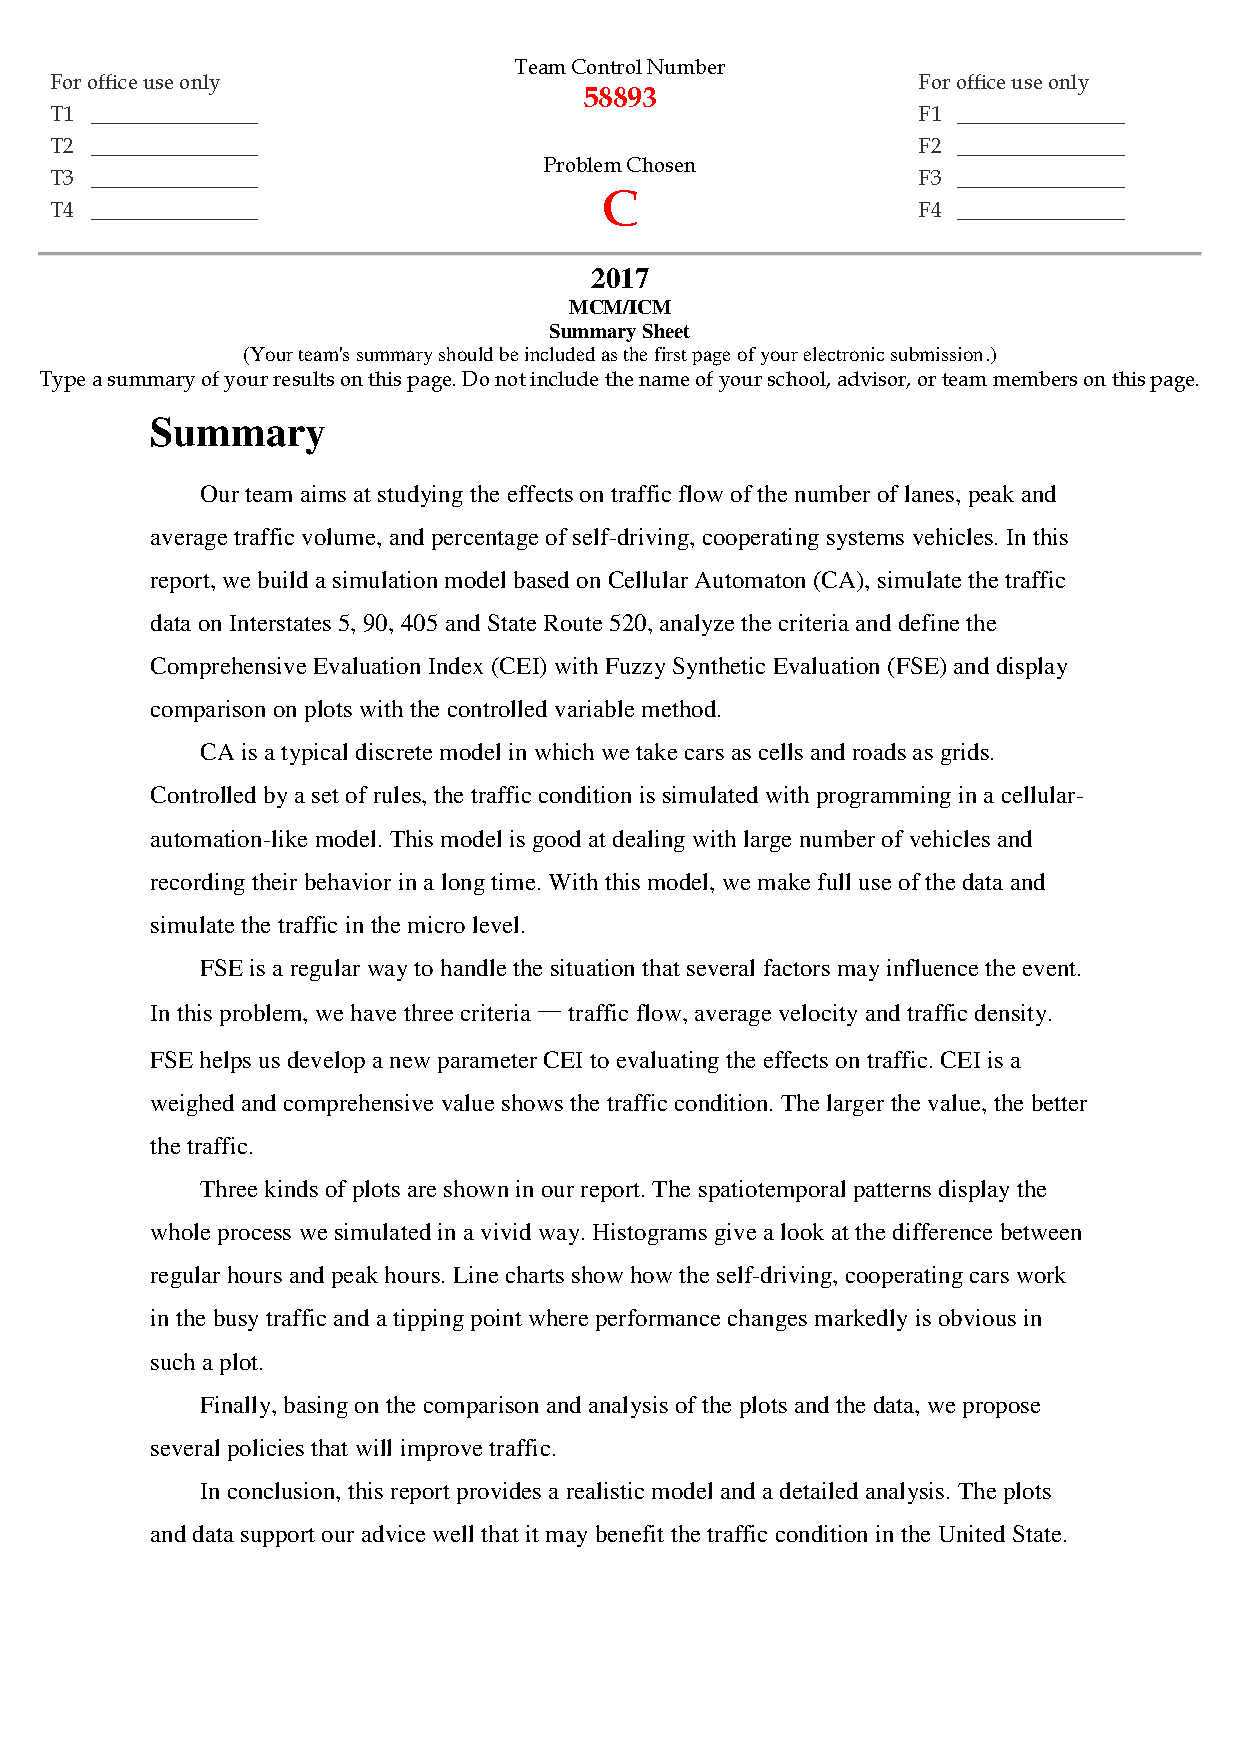
\includepdf{2017Summary.pdf}

	\section{A Letter to the Governor of the State of Washington}
	\begin{spacing}{1.4}
		\begin{flushleft}
			Dear Sir/Madam,
		\end{flushleft}

		We have heard that the governor of the state of Washington are asking of analysis of the effects of allowing self-driving, cooperating cars on the roads listed above in Thurston, Pierce, King, and Snohomish counties. After several days study and consideration, we are glad to submit our solution and we hope that will be good to the traffic condition in United State. Our team has designed a complete model and worked out a series of detailed analysis. We have taken account of various factors that may have effects on the traffic flow including the number of lanes, the peak or average hours and different percentage of vehicles using self-driving, cooperating systems. We also propose policy that will improve traffic and enlarge traffic flow. Our goal is to provide an elaborate plan to include self-driving, cooperating cars in the present traffic and alleviate the traffic pressure under the circumstances that the number of lanes or roads does not change. In this letter, we will introduce a brief view of our modeling approach and the final result to you.

		Here is the modeling approach:
		\begin{enumerate}
			\item The simulation model is based on the principle of the Cellular Automaton.
			\item We first simulate the initial distribution on the whole Interstates 5, 90, and 405, as well as State Route 520. This initial condition is built on the average daily traffic counts in 2015.
			\item We set reasonable rules to control the behavior of the non-self-driving cars on the highway and record its travel parameters.
			\item Cars with self-driving, cooperating system are added by 10\% to 90\% with 20\% interval.
		\end{enumerate}

		The analysis way is as follows:
		\begin{enumerate}
			\item The spatiotemporal pattern is plotted for different percentage of self-driving, cooperating cars to give an approximate view of the whole process.
			\item  The histogram is plotted to show the difference between the regular hours and the peak hours.
			\item  The parameters of the individual cars are calculated into three main factors reflecting the traffic condition: traffic flow, average velocity and traffic density.
			\item  The three main factors are analyzed by Fuzzy Synthetic Evaluation and Comprehensive Evaluation Index is worked out.
			\item  The line chart of Comprehensive Evaluation Index for different percentage of self-driving, cooperating cars shows an elaborate answer to looking for an equilibria and tipping point.
		\end{enumerate}

		Our result shows that the increasing of self-driving, cooperating cars exactly eases the traffic pressure. Under some conditions, dedicating a lane to self-driving, cooperating cars is helpful.

		Hope our solution can alleviate the traffic pressure and make the highway in the United State flows freely.

		\begin{flushleft}
			Yours faithfully,\\
			Team \#58893
		\end{flushleft}

	\end{spacing}


	\newpage
	\tableofcontents
	\newpage

	\section{Introduction}
	Traffic capacity is limited in many regions of the United States because the volume of traffic exceeds the designed capacity of the road networks. Autonomous cars are potential to quadruple capacity of highways without increasing number of lanes or roads. This results in less traffic congestion. Besides, autonomous cars can reduce parking space and traffic accidents, benefit the elderly and the disabled and relieve drivers from commuting hours. Thus, it’s worthy of further analysis.

	\subsection{Restatement of the tasks}
	We are expected to establish a model simulating traffic flow and to analyze the effect of self-driving cooperating cars. Specifically, we decompose the problem into several sub-problems:
	\begin{itemize}
		\item Construct a model that can simulate traffic flow
		\item Form a comprehensive evaluation index indicating the performance under each circumstance
		\item Discuss the influence of the number of lanes
		\item Discuss the influence of peak and average traffic volume
		\item Discuss the influence of percentage of vehicles using self-driving, cooperating systems
		\item Analyze the characteristics of interaction between self-driving and non-self-driving vehicles, including percentage of self-driving vehicles, equilibria, tipping point and exclusively reserved lanes
		\item Design optimization method to enlarge traffic flow
		\item Propose policy that will improve traffic
	\end{itemize}

	\subsection{Assumptions and Justifications}
    To focus on the main problem, we make the following well-justified assumptions.

    \begin{itemize}
\item \textbf{The size of each vehicle is 16 feet $\times$ 6 feet.} Although there are sedan car, van, wagon and SUV, which are of different sizes, we assume that all vehicles on freeways are sedan cars because they are the major components of traffic.
\item \textbf{All the vehicles uniformly accelerate and decelerate.} It is valueless to consider the process of acceleration and deceleration since it has little effect on the traffic flow. We assume a not-self-driving car has constant acceleration ranging from 5 to 7 $mile/h\cdot s$ while a self-driving car has constant acceleration automatically calculated from the distance from the one immediately ahead. Specifically, all vehicles brake at 81576.6 $mile\cdot h^{-2}$.
\item \textbf{The distance between two vehicles tends to maintain some specific value.} We assume that all vehicles are spaced compactly, which means they maintain some minimal safety distance and don’t spread apart. The detailed calculation method of safety distance is shown in Section \ref{sd}. For a not-self-driving vehicle, if the distance from the one immediately ahead is 10\% less than the safety distance, the vehicle decelerates and if the real distance is 10\% more than the safety distance, the vehicle accelerates. For a self-driving vehicle, as long as the real distance is not the same as safety distance, it adjusts its velocity.
\item \textbf{We don’t consider abnormal phenomena.} Accidents, violation of traffic regulations (e.g. speeding) and any other special circumstance are of negligible researching significance in this case.
\item \textbf{Either of the two directions accounts for half of the average daily traffic.} We assume same traffic volume for both sides of the roads.
\item \textbf{Peak traffic hour lasts for approximately an hour.}  According to our experiences in daily life, peak traffic hour usually lasts for an hour. Besides, we know that 8\% of the daily traffic volume occurs during peak travel hours on average. If peak traffic hour lasts for two hours or even longer, then 4.18\% or more of the traffic volume occurs during regular time, which is higher than that of peak hours.
\item \textbf{Not-self-driving cars decelerate randomly.} Without randomization, the model is a deterministic algorithm, i.e., the cars always move in a set pattern once the original state of the road is set, which is not a real-world case. Besides, with randomization, this model can simulate otherwise absent phantom traffic jams \footnotemark \footnotetext{Joseph Stromberg’s explanation of phantom traffic jam is as follows.
\begin{quote}\textit{If there are enough cars on a highway, any minor disruptions to the flow of traffic can cause a self-reinforcing chain reaction: one car brakes slightly, and the ones behind it brake just a bit more to avoid hitting it, with the braking eventually amplifying until it produces a wave of stopped or slowed traffic.}\cite{phantom}\end{quote}}. We set the possibility of deceleration as 0.3.
\item \textbf{Response time for human drivers is approximately 1s.} Humans, unlike self-driving cars, need time to react. Usually, it takes 0.75-1.5s for a driver to take action, so we set the response time as 1s.
\item \textbf{All cars are exactly the calculated safety distance away from the one immediately ahead.} When the model is constructed, we need to input the initial state of the road. We assume all cars are initially well-spaced so that we can better observe the evolution of traffic flow under various circumstances.
\item \textbf{We don’t consider lane changing.} The impact of this phenomenon on traffic flow is negligible compared with that of acceleration and deceleration.
    \end{itemize}


	\subsection{Notations}
    All the variables used in this paper are listed in Table \ref{t1}.

    \begin{table}[H]
    \centering
    \begin{tabular}{lll}
    \toprule
		Symbol & Definition & Units \\
		\midrule
$d$   & the distance between two mileposts, i.e. endMilepost - startMilepost & $mile$ \\
$s$   & stopping distance & $mile$ \\
$l$   & length of a car & $mile$ \\
$v$   & initial velocity of a car & $mile/h$ \\
$c$   & average hourly traffic counts & $1/h$ \\
$a$   & maximum acceleration & $mile/h^2$ \\
$v_{ij,nlane}$ & the average speed of the $j_{th}$ car on the $i_{th}$ section of the freeway which has \textit{nlane} lanes & $mile/h$ \\
$v_{i,nlane}$ & the average speed of all the vehicles on the $i_{th}$ section of the freeway which has \textit{nlane} lanes & $mile/h$ \\
$v_{nlane}$ & the average speed of all the vehicles on the freeway which has \textit{nlane} lanes & $mile/h$ \\
$\rho_{i,nlane}$ & the density of the $i_{th}$ section of the road which has \textit{nlane} lanes & $1/mile$ \\
$\rho_{nlane}$ & the average density of all the sections of the freeway which has \textit{nlane} lanes & $1/mile$ \\
$q_{i,lane}$ & the flow of the $lane_{th}$ lane of the $i_{th}$ section of the freeway which has \textit{nlane} lanes & $1/hour$ \\
$q_{nlane}$ & the average flow of all the sections of the freeway which has \textit{nlane} lanes & $2/hour$ \\
$nlane$ & the number of lanes & $unitless$ \\
${N_i}$ & the total number of vehicles on the $i_{th}$ section of the freeway & $unitless$ \\
$n$   & the number of sections & $unitless$ \\
$n_{i,lane}$ & the number of vehicles on the $lane_{th}$ lane of the $i_{th}$ section of the freeway & $unitless$ \\
$l_i$ & the length of the $i_{th}$ section of the freeway & $mile$ \\
    \bottomrule
    \end{tabular}
    \caption{Symbol Table.}
    \label{t1}
    \end{table}

	\section{Model Design and Justification}
	\subsection{Simulation Model Based on Cellular Automaton}
	Cellular automation is always used for studying the moving objects having varying states in a number of discrete time. In this problem we study, the cellular automation is applied in the following aspects:
	\begin{enumerate}
		\item[$ \bullet $] The ``cell" objects are the travelling cars on the highway.
		\item[$ \bullet $] Each car has its location that the distance from the startMilepost and the lane it drives on are the coordinates.
		\item[$ \bullet $] Each car has a state which is one of moving, accelerating or decelerating.
		\item[$ \bullet $] Each car's state will be affected by a neighborhood which is the former car in different generations according to some rules.
	\end{enumerate}

	The simulation model for this problem has similar rules to the cellular automation that
	$$ \text{vehicle state at time} t=f(\text{former vehicle state at time} (t-1)) $$

	One of the simplest illustration is shown in Figure \ref{generation}. Generation 0 shows the initial state of six cells in the grid. Generation 1 shows the state of these six cells after a period of time. In the simulation model shown later more details will be added in such a basic model like the distance between the two cells and other factors concern in the highway traffic.

	\begin{figure}[H]
		\centering
		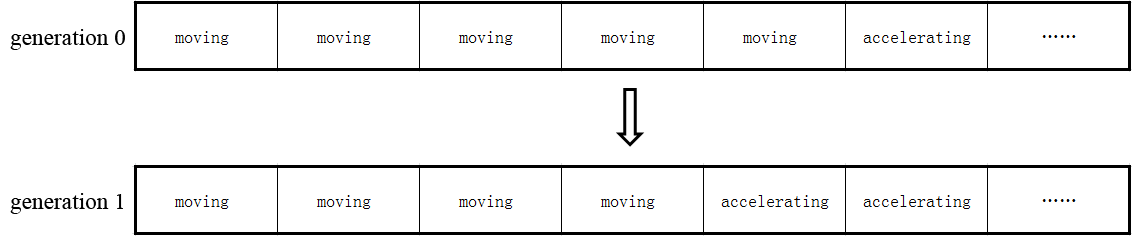
\includegraphics[scale=0.6]{../imgs/generation}
		\caption{A simple illustration for the state changing dependent on time}
		\label{generation}
	\end{figure}



	\subsection{Non-Self-Driving Vehicles Model}
	\subsubsection{Stopping Distance}\label{sd}
	In order to keep safe, we assume the distance between any two vehicles is the stopping distance corresponding to the speed of the latter vehicle. When calculate the stopping distance, two factors are considered — human factors and vehicle factors.


	For the human part, there are two components — the human perception time which is the time needed for human to see the hazard and the human reaction time during which the brain convey the signal to the body. The human perception time ranges from 0.25 second to 0.5 second while the human reaction time varies from 0.25 second to 0.75 second.\cite{stopping} For convenience, we take the sum of these two parts as 1 second.

	For the vehicle part, the braking distance concerns the maximum acceleration. We take the braking distance for vehicles at speed 100 kilometer per hour as 32 meters. The maximum acceleration is calculated then:
	$$ a=\dfrac{(100\ km\cdot h^{-1})^2}{2\times 38\ m}=10.13\ m\cdot s^{-2}=81576.6\ mile\cdot h^{-2} $$
	here we use mile per hour for the convenience of the subsequent calculation.

	Then the stopping distance related to the velocity of the vehicle is achieved:
	$$ s=\dfrac{v^2}{2a}+\dfrac{v}{3600}\ mile $$
	where $ v $ is the velocity of the latter vehicle and $ a $ is the maximum acceleration $ 81576.6\ mile\cdot h^{-2} $.

	Note that when the velocity is small enough it is no need to keep the stopping distance above. The main reason is the reaction time will be shortened. We assume the stopping distance is 4 feet as the velocity is below 18.75 mile per hour.

	In this model, every vehicle will maintain the exact stopping distance with the former one corresponding to its velocity. The means, while the distance is smaller than the theoretical value, the vehicle will slow down and vice versa. The maximum velocity is limited to 60 mile per hour.

	\subsubsection{Initial Distribution}
	The initial condition is affected by the traffic counts and the number of lanes.

	We first consider the average hourly traffic counts. Since we know the average daily traffic counts (2015) and 8\% of the daily traffic volume occurs during peak travel hours. We set the peak travel hour is one hour every day and in this period $$ c=\text{average daily traffic counts}\times 8\% $$ In the other hours, the traffic acounts is  $$ c=\text{average daily traffic counts}\times (1-8\%)/24=\text{average daily traffic counts}\times 4\%  $$

	We know $ \dfrac{d}{s+l}\cdot n $ is the traffic counts between two mileposts in $ \dfrac{d}{v} $ hours. Then we achieve the equation:
	$$ \dfrac{d}{s+l}\cdot n\cdot\frac{1}{\frac{d}{v}}=c\implies vn=(s+l)c $$

	We have $ s=\dfrac{v^2}{2a}+\dfrac{v}{3600}\ mile $ and $ l=16\ ft=0.003\ mile $. After simplification, we have
	$$ \dfrac{c}{2a}\cdot v^2+\left(\dfrac{c}{3600}-n\right)\cdot v+0.003=0 $$
	$$ s+l=\dfrac{v^2}{2a}+\dfrac{v}{3600}+0.003 $$

	We use these two equations to determine the initial distribution on the highway. With known average hourly traffic counts and number of the lanes, the initial velocity of a car can be solved, leading to the stopping distance. Initially, there will be $ \dfrac{d}{l+s} $ cars on every lane in this section of the highway and $ l+s $ is the distance from the head of the former car and the head of the latter one. All the vehicles on this section of the highway will start to move with the initial speed.

	\subsubsection{Control Ruleset}
	After the initial condition is set, we can simulate all the cars under the control rules and record the parameters of every cars including location, acceleration and velocity. These parameters can be used to calculate the average velocity, traffic flow and density of the cars in any section of the highway in future analysis. Here the control ruleset is as follows:
	\begin{itemize}
		\item Every vehicle adjusts the velocity by accelerating or decelerating according to the distance between the former car and itself. When the distance is 10\% longer than the stopping distance of its velocity, the vehicle will accelerate. Similarly, it will decelerate when the distance is 10\% shorter. 60 mile per hour is the maximum velocity.
		\item The average daily traffic counts vary among different sections of a highway. This is caused by the difference between the number of the entering cars and the one of the leaving ones. This distinct values of the average daily traffic counts lead to different average velocity in different sections. As the first car of the latter section drives to the last car of the former section, it may have to change its velocity so that it can adapt the traffic condition in the new section. And its change of velocity will affect the state of the following vehicles and leads to a domino effect.
		\item  Since every car is driven by a real human, there should be a randomization deceleration during the process of driving. This will also leads to a domino effect and slow down the cars behind it.
	\end{itemize}

	\subsection{Self-Driving Vehicles Model}
	\subsubsection{Initial Condition}
	In order to give a clearer comparison with the Non-Self-Driving Vehicles Model, the initial condition doesn't change in this section. This means there will be $ \dfrac{d}{l+s} $ cars on every lane in this section of the highway and $ l+s $ is the distance from the head of the former car and the head of the latter one. All the vehicles on this section of the highway will start to move with the initial speed. The distance and the initial speed are calculated by the formula in Non-Self-Driving Vehicles Model.

	With the different control ruleset for self-driving vehicles, the simulation will show the real-time traffic situation with different percentage of self-driving cars after a period of time.

	\subsubsection{Control Ruleset}
	Due to various sensers and coorperating system on the self-driving vehicles, they can make more precise decisions and the ruleset is different from the human-driving one. Also, self-driving vehicles are more accurate.
	\begin{itemize}
		\item \textbf{There exists interaction between selfdriving
		and non-self-driving vehicles.} The self-driving vehicles don't have a reaction time. When a self-driving vehicle drives behind a non-self-driving vehicle, we suppose the senser can obtain the infromation about the velocity of the former vehicle and the distance between the two vehicles. And to prevent the sudden action of the human-driving vehicle, the vehicle has to keep a stopping distance according to its velocity: $ s=\dfrac{v^2}{2a} $.
		\item \textbf{There exists cooperation between self-driving cars.} When the former vehicle is another self-driving vehicle, the two vehicles can cooperate. Since we are not designing a self-driving car, we omit the detailed velocity changing in the first period of time. We set another standard for the stopping distance and call it safe distance $ s_c $. A safe range is assumed around $ s_c $. The safe distance and the safe range for different velocity is shown in Table \ref{range}.

		\begin{table}[H]
			\centering
			\begin{tabular}{cccc}
				\toprule
				velocity[mile/h] & $ 0\sim20 $  & $ 20\sim40 $ & $ 40\sim60 $ \\
				\midrule
				Safe Distance $ s_c $[feet]  & 4     & 29    & 84 \\
				Safe Range[feet] & $ 0\sim4 $  & $ 4\sim54 $ & more than $ 49 $ \\
				\bottomrule
			\end{tabular}%
			\caption{The relation between the safe distance, the safe range and velocity}
			\label{range}%
		\end{table}%

		An example about how this works is shown as follows:

		For any two self-driving vehicles, if the velocity of the two vehicles both fall on $ 20\sim 40\  mile/h $ and the distance between two cars falls on the corresponding safe range, here it is $ 4\sim54\  feet$, after a period of time, the distance is set as the safe distance. At first, the latter car will accelerate with the origin acceleration we assume. In the last 0.1 second, it somehow adjust the distance as the safe distance as well as make their velocity the same, which is called a stable situation. In this process, we omit how the self-driving change its acceleration and adjust the distance but focus on the stable situation. As the stable situation is reached, with cooperation, the latter vehicle can just copy the action of the former one until their velocity no longer falls on $ 20\sim 40\  mile/h $, then they change velocity and approach another stable situation. If the distance between the two cars does not fall on the corresponding safe range, the latter vehicle travels with a constant acceleration until the distance enters the safe range.
	\end{itemize}



	\section{Results}
	\subsection{Influencing factors}
	%时空斑图

	\subsubsection{Variables and Criteria}
There are three variables: number of lanes, peak and/or average traffic volume, and percentage of vehicles using self-driving, cooperating systems. We need a comprehensive evaluation index to indicate the performance on different conditions, so we propose the following criteria:
\begin{itemize}
\item \textbf{Average speed ($v$)}: the average speed of all vehicles driving on highways with a specific number of lanes over an hour.
	$$v_{i,nlane}=\dfrac{\sum\limits_{j=1}^{N_i}v_{ij,nlane}}{{N_i}}$$
	$$v_{nlane}=\dfrac{\sum\limits_{i=1}^nv_{i,nlane}\times l_i}{\sum\limits_{i=1}^nl_i}$$
	where $v_{ij,nlane}$ stands for the average speed of the $j_{th}$ car on the $i_{th}$ section of the freeway which has \textit{nlane} lanes, $v_{i,nlane}$ stands for the average speed of all the vehicles on the $i_{th}$ section of the freeway which has \textit{nlane} lanes and $v_{nlane}$ stands for the average speed of all the vehicles on the freeway which has \textit{nlane} lanes. ${N_i}$ and $n$ stands for the total number of vehicles on the $i_{th}$ section of the freeway and the number of sections. $l_i$ stands for the length of the $i_{th}$ section of the freeway.

\item \textbf{Density ($\rho$)}: the total number of vehicles per unit length of the freeway.
$$\rho_{i,nlane}=\dfrac{\sum\limits_{lane=1}^{\#lane}n_{i,lane}}{l_i}$$
$$\rho_{nlane}=\dfrac{\sum\limits_{i=1}^{n}\rho_{i,nlane}}{n}$$
where $n_{i,lane}$ stands for the number of vehicles on the $lane_{th}$ lane of the $i_{th}$ section of the freeway, $\rho_{i,nlane}$ stands for the density of the $i_{th}$ section of the road which has \textit{nlane} lanes and $\rho_{nlane}$ stands for the average density of all the sections of the freeway which has \textit{nlane} lanes.

\item \textbf{Flow ($q$)}: the total number of vehicles passing a milepost per hour.
$$q_{i,nlane}=\sum\limits_{lane=1}^{\#lane}q_{i,lane}$$
$$q_{nlane}=\dfrac{\sum\limits_{i=1}^{n}q_{i,nlane}}{n}$$
where $q_{i,lane}$ stands for the flow of the $lane_{th}$ lane of the $i_{th}$ section of the freeway which has \textit{nlane} lanes and $q_{nlane}$ stands for the average flow of all the sections of the freeway which has \textit{nlane} lanes.
\end{itemize}

	\subsubsection{Percentage of the vehicles using self-driving cars and number of lanes}%折线图
	In order to show the effects on the traffic of the percentage of the self-driving, cooperating cars and the number of the lanes, we plot the line charts to show the tendence of the three parameters with the change of these two variables.

	In Figure \ref{all_1}, we can have a look at the relation between the velocity and these two variables. Along the x-axis, it shows the different persentage. The self-driving, cooperating cars exactly do good to the traffic condition. We found that the effects of this new kind of cars increase almost linear from 10\% to 90\% and reaches a maximum at 90\%. And it shows a decreasement from 90\% to 100\%. This figure also shows that two lanes may cause a low average velocity and five landes a high average velocity if other conditions do not change. And the difference is not obvious between three and four lanes.

	\begin{figure}[H]
		\centering
		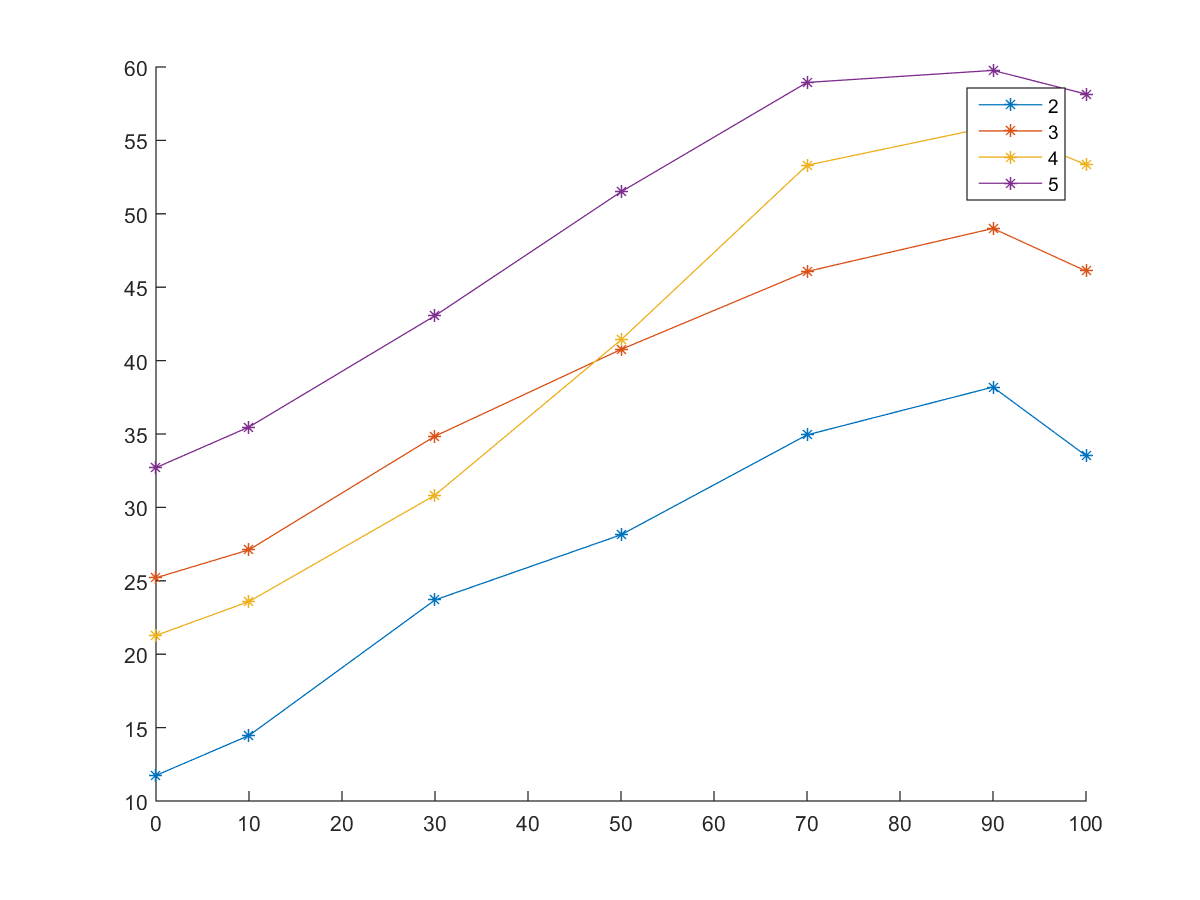
\includegraphics[scale=0.5]{../imgs/all_1}
		\caption{Relation between the velocity and the percentage of the self-driving, cooperating cars and the number of the lanes}
		\label{all_1}
	\end{figure}

	In Figure \ref{all_2}, we can have a look at the relation between the flow and these two variables. Again, the self-driving, cooperating cars exactly do good to the traffic condition.  We found that the effects of this new kind of cars increase almost linear from 10\% to 90\%. For lanes 3,4 and 5, there is a tipping point where performance changes markedly from 90\% to 100\%. However for 2 lanes condition, 90\% to 100\% contribute little to increase the flow. This figure also shows the more lanes can afford more traffic flow which is understandable.

	\begin{figure}[H]
		\centering
		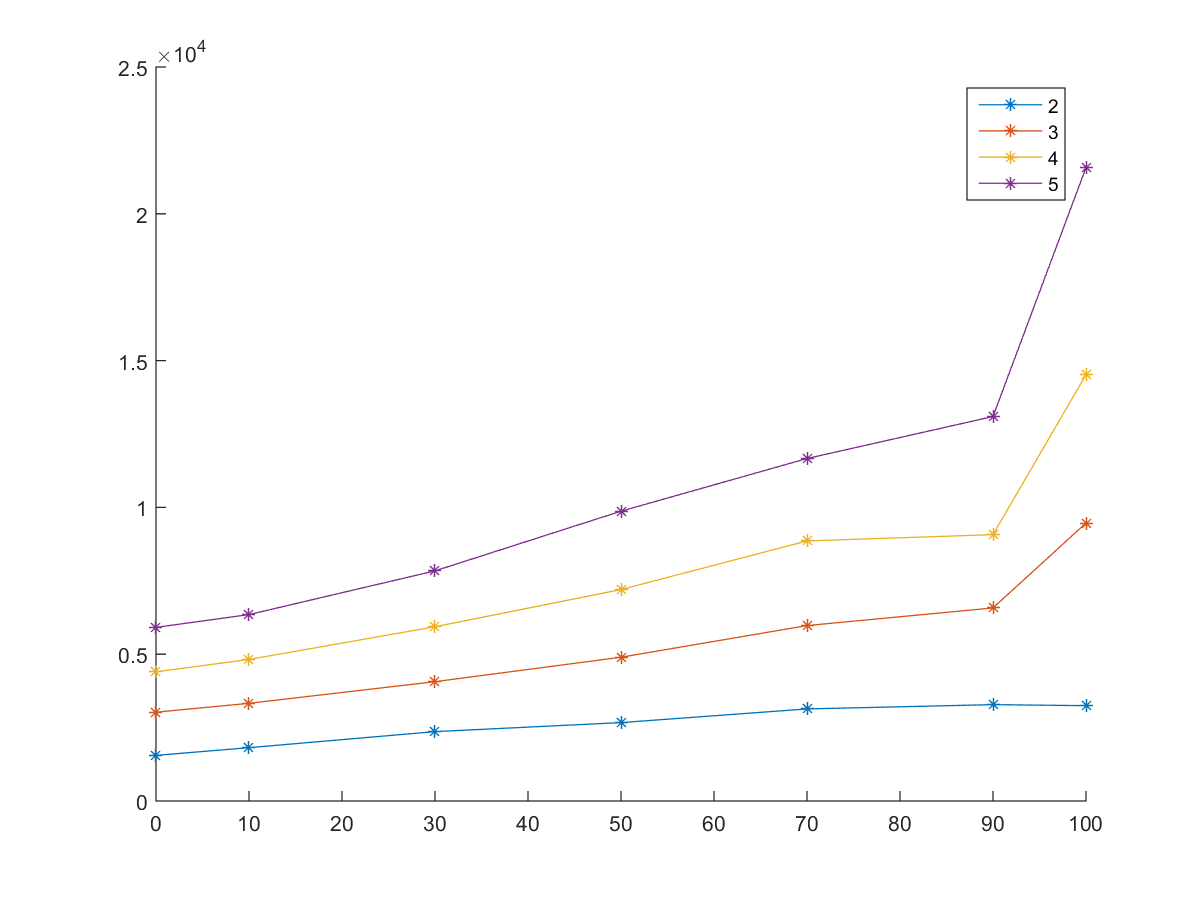
\includegraphics[scale=0.5]{../imgs/all_2}
		\caption{Relation between the flow and the percentage of the self-driving, cooperating cars and the number of the lanes}
		\label{all_2}
	\end{figure}

	In Figure \ref{all_3}, we can have a look at the relation between the density and these two variables. Since the lower density shows better traffic condition, the self-driving, cooperating cars exactly do good to the traffic condition.  We found that the effects of this new kind of cars increase almost linear from 10\% to 100\% for lanes 3 and 4. For 2 lanes, the difference between 90\% and 100\% makes tiny efforts to the density. For 5 lanes, there is a tipping point where performance changes markedly from 90\% to 100\%. This figure shows in 2-lane-road and 5-lane-road the density is lower while in 3-lane-road and 4-lane-road the density is higher.

	\begin{figure}[H]
		\centering
		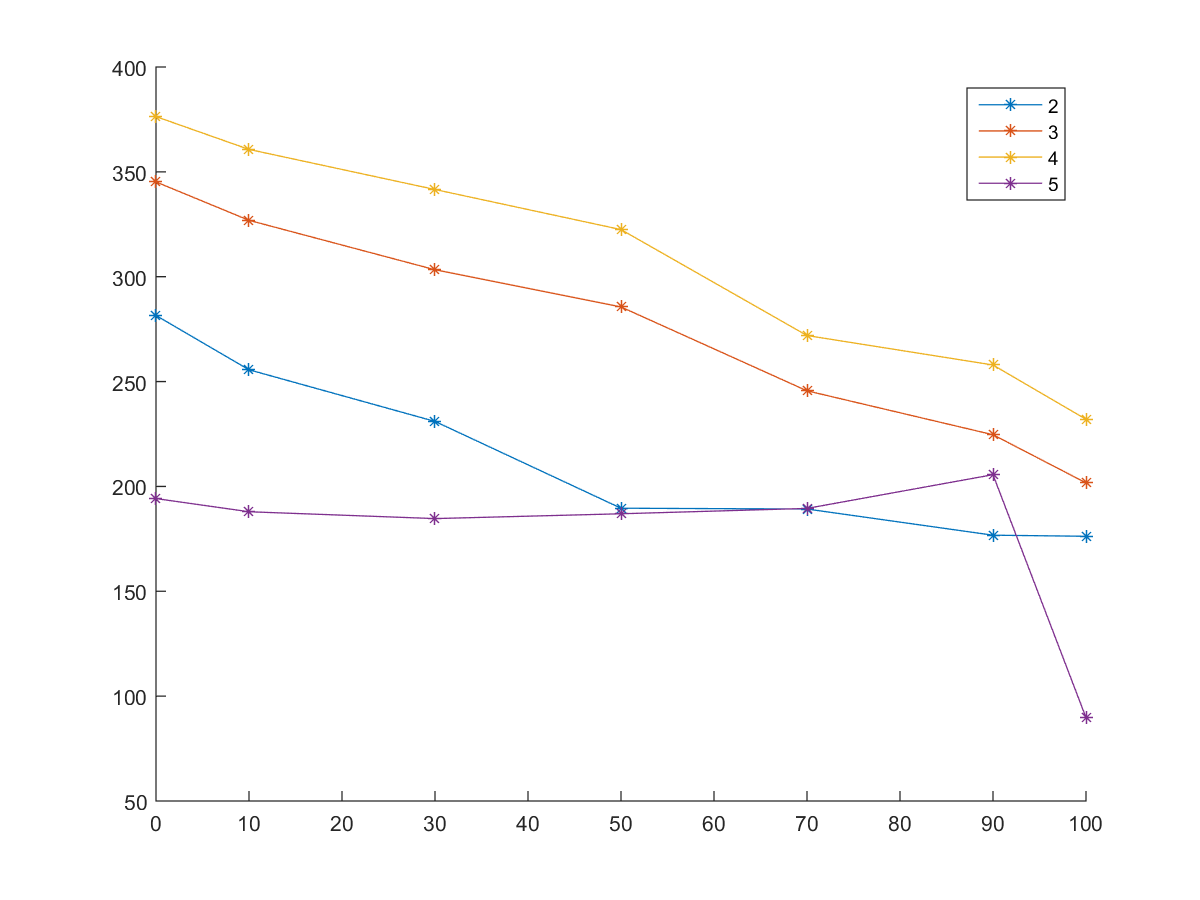
\includegraphics[scale=0.5]{../imgs/all_3}
		\caption{Relation between the density and the percentage of the self-driving, cooperating cars and the number of the lanes}
		\label{all_3}
	\end{figure}



	\subsubsection{Peak and/or average traffic volume }%直方图
	In order to show the effects on the traffic of the percentage of the self-driving, cooperating cars and period of time, peak and/or average traffic volum, we plot the bar graphs to show the tendence of the three parameters with the change of these two variables.

	In Figure \ref{all_bar_1}, we can have a look at the relation between the velocity and these two variables. The self-driving, cooperating cars do good to the traffic condition only in peak hours. We found that in peak hours, the effects of this new kind of cars increase almost linear from 10\% to 70\% and reaches a maximum at 90\%. In regular times, almost all the vehicle has a speed of 60 mile per hour.

	\begin{figure}[H]
		\centering
		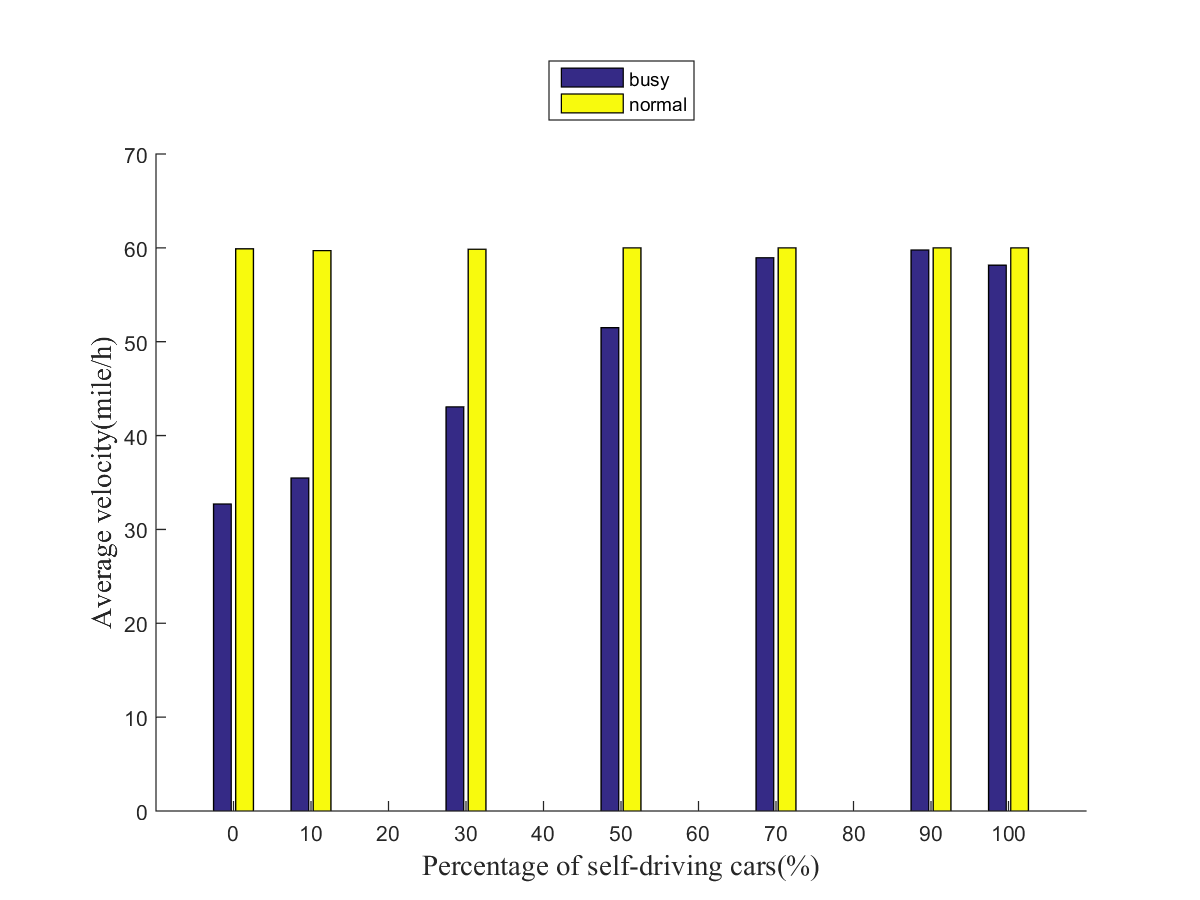
\includegraphics[scale=0.5]{../imgs/all_bar_1}
		\caption{Relation between the velocity and the percentage of the self-driving, cooperating cars and period of time}
		\label{all_bar_1}
	\end{figure}

	In Figure \ref{all_bar_2}, we can have a look at the relation between the flow and these two variables. The self-driving, cooperating cars do good to the traffic condition only in peak hours. We found that in peak hours, the effects of this new kind of cars increase almost linear from 10\% to 90\% and has a tipping point a 100\%. In regular times, the flow is confined by the indeed volume vehicle, thus it shows no relation for the change of the percentage of self-driving cars.

	\begin{figure}[H]
		\centering
		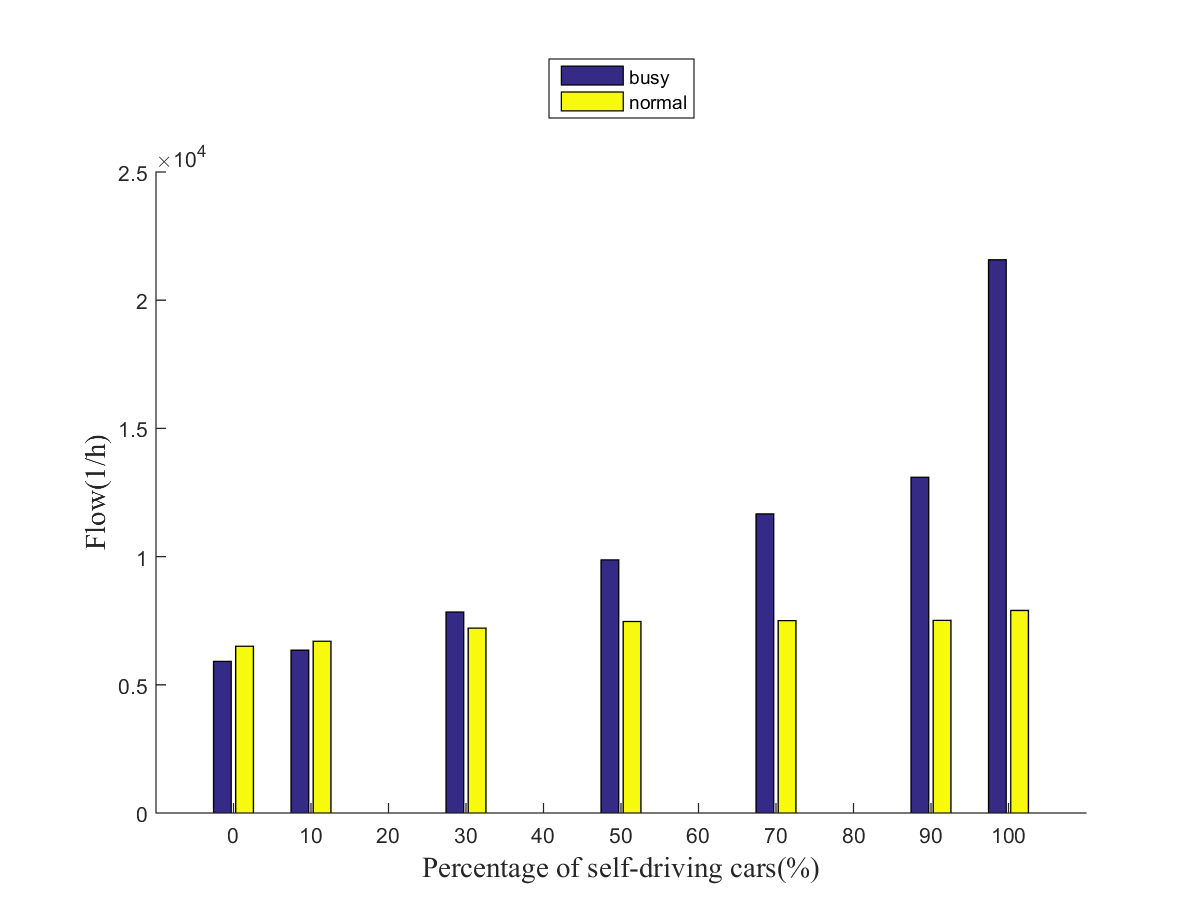
\includegraphics[scale=0.5]{../imgs/all_bar_2}
		\caption{Relation between the flow and the percentage of the self-driving, cooperating cars and period of time}
		\label{all_bar_2}
	\end{figure}

	In Figure \ref{all_bar_3}, we can have a look at the relation between the density and these two variables. The self-driving, cooperating cars do good to the traffic condition. We found that in peak hours, the effects of this new kind of cars increase almost linear from 10\% to 100\%. In regular times, the density is determined by the indeed volume of vehicles, thus it shows no relation for the change of the percentage of self-driving cars.

	\begin{figure}[H]
		\centering
		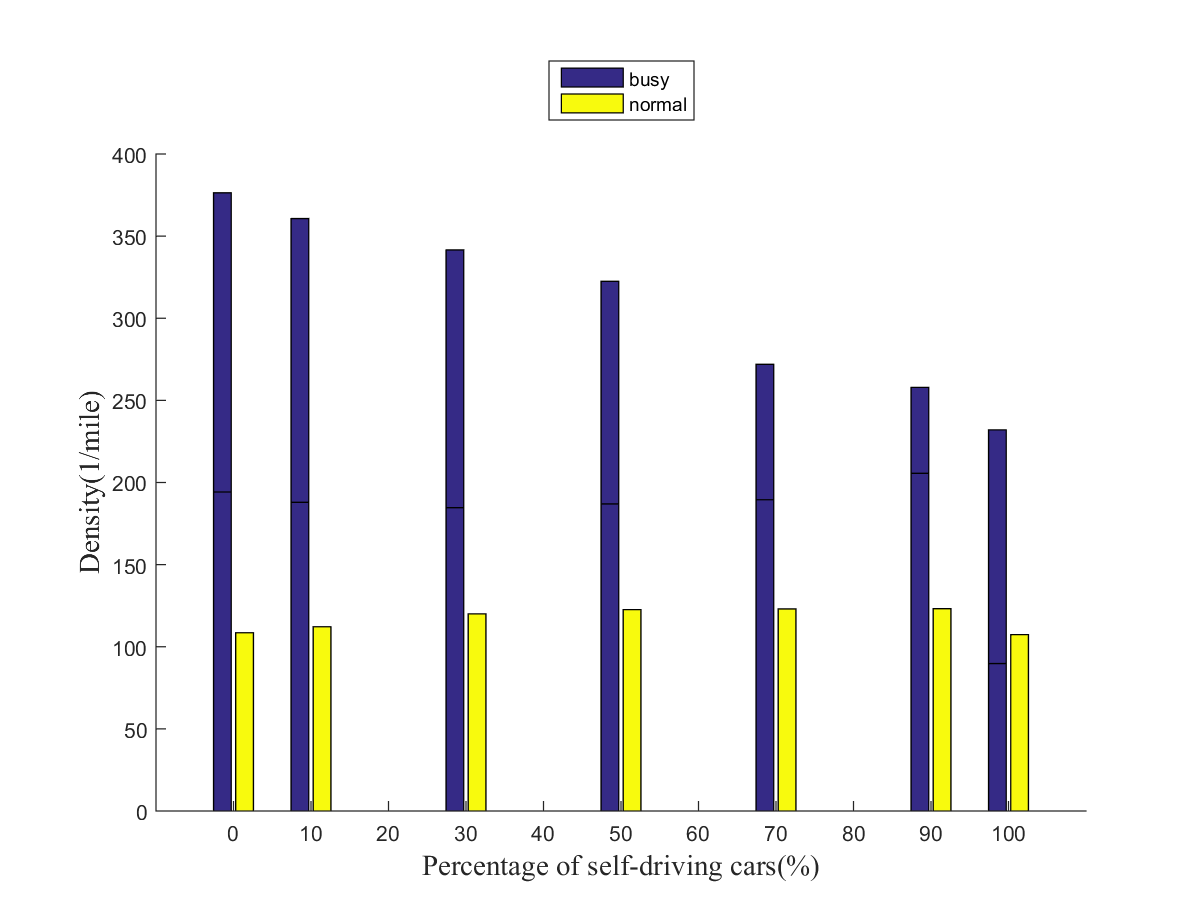
\includegraphics[scale=0.5]{../imgs/all_bar_3}
		\caption{Relation between the density and the percentage of the self-driving, cooperating cars and period of time}
		\label{all_bar_3}
	\end{figure}

	\subsection{Optimal situation investigation}
	\subsubsection{Comprehensive Evaluation Index}
	In order to examine under what conditions, a lane should be dedicated to self-driving cars, we first need a specific comprehensive evaluation index to quantify the traffic flow, and then we can compare the variations after we reserve one lane exclusively for self-driving cars and determine whether this action is beneficial. Since we have quantitative information about the traffic flow (i.e. the average speed, density and flow), we don’t need to rely on Analytic Hierarchy Process (AHP), which is relatively subjective. We implement fuzzy synthetic evaluation (FSE)\cite{fse}. FSE is a multiple-criteria-decision-making method proposed by American mathematician and computer scientist Lotfi A. Zadeh. It can determine the weights of each variable and obtain one uniquely determined weighted score of each situation. We use this technique to analyze the performance under different scenarios.

	Below we use the traffic flow at peak hours when there are 50\% self-driving vehicles as an example. Other situations can be processed in a similar way.

	\textbf{Collect attributes data for all variables}

	Three variables are considered in our model: average speed, density and flow. The variables are the number of lanes: 2, 3, 4 and 5. The values of each attribute of each variable are listed in the table below.

	All the data of B and H are listed in the table below.
\begin{table}[H]
	\begin{center}
		\begin{tabular}{c|ccc}
		\hline
		\# of lanes & $v$   & $\rho$ & $q$ \\
		\hline
		2     & 28.13  & 2670.12  & 189.61  \\
		3     & 40.76  & 4896.78  & 285.58  \\
		4     & 41.41  & 7201.30  & 322.48  \\
		5     & 51.50  & 9870.94  & 186.96  \\
		\hline
		\end{tabular}
	\caption{Attributes data for all variables.}
	\end{center}
\end{table}


	\section{Sensitivity Analysis}
	\subsection{Probability of Random Deceleration}
	In the simulation, we suppose the probability of random deceleration is 0.3. Indeed, we find little information about it. Since the random deceleration depends on human behavior which may be influenced by people's feeling, weather, surroundings and many other uncontrollable factors, it is hard to be determined and adapt to all the circumstances. If the probability is raised, it adds to the traffic condition and vice versa.
	\subsection{Choice of Acceleration}
	There are two kinds of acceleration in this model. One is the maximum acceleration which is used for calculation of the stopping distance. This acceleration is achieved by information from website\cite{stopping}. However, it is still an approximate value which affected by the performance of the vehicles, the road condition like down hill or snow and ice. Another acceleration is the usual acceleration which is randomly chosen from 5 to 7 $ mile\cdot h\cdot s $. This is also determined from the website\cite{acc}. In this model, the choice of acceleration and deceleration is the same, but in fact, acceleration is related to the motor while deceleration is related to the brake. If the acceleration is raised, it helps to increase the traffic flow.
	\subsection{Reaction Time}
	The reaction time ranges from 0.5 to 1.25 second.\ref{sd} To make an overall consideration, we choose 1 second as the reaction time. The longer reaction time leads to harder traffic condition.
	\section{Strengths and Weaknesses}
	\subsection{Strengths}
	\begin{itemize}
		\item \textbf{Considering various kinds of factors. }Our model takes the effects on traffic flow of the number of lanes, peak and average traffic volume and percentage of self-driving, cooperating vehicles into account.
		\item \textbf{Analyzing large amount of data. }Our model analyzes the traffic condition on Interstates 5, 90 and 405, as well as State Route 520. Hundreds of sections of highway that each section is road between two Milepost and tens of millions of vehicles are simulated.
		\item \textbf{Making detailed analysis. }Our model provides information about traffic flow, average velocity and traffic density of sections of the highway. Besides the spatiotemporal patterns histograms and line charts, we also use FSE to combine the three criteria and produce a new criterion Comprehensive Evaluation Index to show the comprehensive evaluation of the traffic condition under different circumstances. These analysis bring about an optimization method to enlarge traffic flow and improve traffic.
	\end{itemize}
	\subsection{Weakness}
	\begin{itemize}
		\item \textbf{No lane changing.} Due to time limit, we have not taken lane changing into account which means there is no overtaking in the whole process no matter for self-driving or human-driving vehicles. Overtaking may aggravate the traffic condition in the busy traffic. More seriously, the new-entering cars won't change their lanes which means the entering lane may be much more busy than other lanes if the traffic flow is huge.
		\item \textbf{Cancelling between the entering and leaving cars.} Since we do not have the number for the entering and leaving cars on each section of the highway, we simply consider that the traffic counts of one section is the sum of the previous section and the entering ones or the difference between the previous one and the leaving ones. This means some traffic volume is cancelled under this hypothesis. These traffic volume makes the traffic worse in the real world.
	\end{itemize}






	\newpage

	\begin{thebibliography}{0}
		\bibitem{stopping} Neilsen, Joel. ``Stopping Distance", Safe Drive Training,  \url{<http://sdt.com.au/safedrive-directory-STOPPINGDISTANCE.htm>.} Accessed 21 January 2017.
		\bibitem{} Shiffman, Daniel. ``Cellular Automata", \textit{The Nature of Code}, Lightning Source Inc, 2008. 323-354. Print.
		\bibitem{phantom} Stromberg, Joseph. ``Why do traffic jams sometimes form for no reason?", Vox, \url{< http://www.vox.com/2014/11/24/7276027/traffic-jam>.} Accessed 22 January 2017.
		\bibitem{acc} Consumer Reports, ``Best \& Worst Car Acceleration", Consumer Reports, \url{<http://www.consumerreports.org/cro/news/2012/05/best-worst-acceleration/index.htm>.} Accessed 23 January 2017.
	\end{thebibliography}








	\newpage

\section*{Appendix}
\subsection*{CMakeLists.txt}
\lstset{language=CMake}
\lstinputlisting{../CMakeLists.txt}


\subsection*{C++ Code}
\lstset{language=C++}
\lstinputlisting{../src/mcm.h}
\lstinputlisting{../src/Car.h}
\lstinputlisting{../src/Car.cpp}
\lstinputlisting{../src/HumanCar.h}
\lstinputlisting{../src/HumanCar.cpp}
\lstinputlisting{../src/AutoCar.h}
\lstinputlisting{../src/AutoCar.cpp}
\lstinputlisting{../src/Layout.h}
\lstinputlisting{../src/Layout.cpp}
\lstinputlisting{../src/main.cpp}


\subsection*{MATLAB Code}
\lstset{language=Matlab}
\lstinputlisting{../matlab/readData.m}
\lstinputlisting{../matlab/parseData.m}
\lstinputlisting{../matlab/drawSingle.m}
\lstinputlisting{../matlab/drawBar.m}
\lstinputlisting{../matlab/main.m}



\end{document}

